\chapter{Two Processors}
\label{chap:p2}

\section{Profiles}
\label{sec:p2-profiles}

\todo{Prove that same profiles have same runtime.}

If one considers the problem of scheduling an intree onto two processors, it becomes clear that HLF is optimal (\todo{Proof.}). \todo{Is the following correct:} Moreover, we can conclude that we can compute the optimal expected finish time in polynomial time.

This section shows how the original problem of an intree DAG can be mapped onto another, more compact structure.

\subsection{Profiles of Intrees}
\label{sec:p2-simple-method-runtime-profiles-for-intrees}

If we consider the trees in figure \ref{fig:p2-four-intrees-with-same-profile-6-3-1}, we can compute that for two processors HLF always yields an expected run time of $\frac{49}{8}$ for each of them, which is optimal:

\begin{figure}[ht]
  \centering
  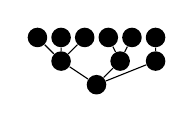
\begin{tikzpicture}[scale=.2]
\node[circle, scale=0.75, fill] (tid0) at (4.5,1.5){};
\node[circle, scale=0.75, fill] (tid1) at (2.25,3){};
\node[circle, scale=0.75, fill] (tid4) at (0.75,4.5){};
\node[circle, scale=0.75, fill] (tid5) at (2.25,4.5){};
\node[circle, scale=0.75, fill] (tid6) at (3.75,4.5){};
\draw[](tid1) -- (tid4);
\draw[](tid1) -- (tid5);
\draw[](tid1) -- (tid6);
\node[circle, scale=0.75, fill] (tid2) at (6,3){};
\node[circle, scale=0.75, fill] (tid7) at (5.25,4.5){};
\node[circle, scale=0.75, fill] (tid8) at (6.75,4.5){};
\draw[](tid2) -- (tid7);
\draw[](tid2) -- (tid8);
\node[circle, scale=0.75, fill] (tid3) at (8.25,3){};
\node[circle, scale=0.75, fill] (tid9) at (8.25,4.5){};
\draw[](tid3) -- (tid9);
\draw[](tid0) -- (tid1);
\draw[](tid0) -- (tid2);
\draw[](tid0) -- (tid3);
\end{tikzpicture}
%%% Local Variables:
%%% TeX-master: "thesis/thesis.tex"
%%% End: \hspace{0.5cm}
  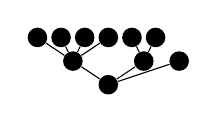
\begin{tikzpicture}[scale=.2]
\node[circle, scale=0.75, fill] (tid0) at (5.25,1.5){};
\node[circle, scale=0.75, fill] (tid1) at (3,3){};
\node[circle, scale=0.75, fill] (tid4) at (0.75,4.5){};
\node[circle, scale=0.75, fill] (tid5) at (2.25,4.5){};
\node[circle, scale=0.75, fill] (tid6) at (3.75,4.5){};
\node[circle, scale=0.75, fill] (tid7) at (5.25,4.5){};
\draw[](tid1) -- (tid4);
\draw[](tid1) -- (tid5);
\draw[](tid1) -- (tid6);
\draw[](tid1) -- (tid7);
\node[circle, scale=0.75, fill] (tid2) at (7.5,3){};
\node[circle, scale=0.75, fill] (tid8) at (6.75,4.5){};
\node[circle, scale=0.75, fill] (tid9) at (8.25,4.5){};
\draw[](tid2) -- (tid8);
\draw[](tid2) -- (tid9);
\node[circle, scale=0.75, fill] (tid3) at (9.75,3){};
\draw[](tid0) -- (tid1);
\draw[](tid0) -- (tid2);
\draw[](tid0) -- (tid3);
\end{tikzpicture}
%%% Local Variables:
%%% TeX-master: "thesis/thesis.tex"
%%% End: \hspace{0.5cm}
  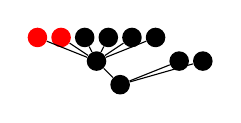
\begin{tikzpicture}[scale=.2]
\node[circle, scale=0.75, fill] (tid0) at (6,1.5){};
\node[circle, scale=0.75, fill] (tid1) at (4.5,3){};
\node[circle, scale=0.75, fill, red] (tid4) at (0.75,4.5){};
\node[circle, scale=0.75, fill, red] (tid5) at (2.25,4.5){};
\node[circle, scale=0.75, fill] (tid6) at (3.75,4.5){};
\node[circle, scale=0.75, fill] (tid7) at (5.25,4.5){};
\node[circle, scale=0.75, fill] (tid8) at (6.75,4.5){};
\node[circle, scale=0.75, fill] (tid9) at (8.25,4.5){};
\draw[](tid1) -- (tid4);
\draw[](tid1) -- (tid5);
\draw[](tid1) -- (tid6);
\draw[](tid1) -- (tid7);
\draw[](tid1) -- (tid8);
\draw[](tid1) -- (tid9);
\node[circle, scale=0.75, fill] (tid2) at (9.75,3){};
\node[circle, scale=0.75, fill] (tid3) at (11.25,3){};
\draw[](tid0) -- (tid1);
\draw[](tid0) -- (tid2);
\draw[](tid0) -- (tid3);
\end{tikzpicture}
%%% Local Variables:
%%% TeX-master: "thesis/thesis.tex"
%%% End: \hspace{0.5cm}
  \begin{tikzpicture}[scale=.2]
\node[circle, scale=0.75, fill] (tid0) at (5.25,1.5){};
\node[circle, scale=0.75, fill] (tid1) at (2.25,3){};
\node[circle, scale=0.75, fill, task_scheduled] (tid4) at (0.75,4.5){};
\node[circle, scale=0.75, fill] (tid5) at (2.25,4.5){};
\node[circle, scale=0.75, fill] (tid6) at (3.75,4.5){};
\draw[](tid1) -- (tid4);
\draw[](tid1) -- (tid5);
\draw[](tid1) -- (tid6);
\node[circle, scale=0.75, fill] (tid2) at (6.75,3){};
\node[circle, scale=0.75, fill, task_scheduled] (tid7) at (5.25,4.5){};
\node[circle, scale=0.75, fill] (tid8) at (6.75,4.5){};
\node[circle, scale=0.75, fill] (tid9) at (8.25,4.5){};
\draw[](tid2) -- (tid7);
\draw[](tid2) -- (tid8);
\draw[](tid2) -- (tid9);
\node[circle, scale=0.75, fill] (tid3) at (9.75,3){};
\draw[](tid0) -- (tid1);
\draw[](tid0) -- (tid2);
\draw[](tid0) -- (tid3);
\end{tikzpicture}
%%% Local Variables:
%%% TeX-master: "thesis/thesis.tex"
%%% End: 
  \caption{Four intrees with the same profile ($\profile{6,3,1}$). All of them have expected run time of $49/8$ if scheduled with HLF on two processors.}
  \label{fig:p2-four-intrees-with-same-profile-6-3-1}
\end{figure}

The intrees in figure \ref{fig:p2-four-intrees-with-same-profile-6-3-1} have the following in common: At each level, they have the same amount of tasks (six tasks at the topmost level, three in the middle one and one at the bottom level).

We can use the number of tasks per level as a (non-bijective) ``encoding'' of intrees. For now, we call this encoding a \emph{profile} of the intree. The above intrees would all be encoded as a profile containing the numbers 6, 3 and 1 in that order. We denote the profile by $\profile{6, 3, 1}$.

Note that not all sequences of numbers can be used as profiles. In particular, the last number in a profile is (w.l.o.g.) 1 (since we have only one task as the root of the tree)\footnote{This, of course, introduces some overhead in notation, but we leave it as it is since it is easier to read this way.}. Moreover, it can not be the case that there is a zero in a profile (since this would imply that there is \emph{no task} on one specific level in the intree).

Moreover, we introduce a abbreviating notation for profiles.

\begin{definition}[Compact notation of profiles]
  For a profile $p$, we introduce a shorthand notation that groups successive ones. That is, instead of writing $j$ consecutive ones, we simply write $\profileones{j}$.
\end{definition}

As a simple example, we rewrite $\profile{2,1,1,1,5,2,1,1,1,1,1,2,1}$ as 
$\profile{2,\profileones{3},5,2,\profileones{5},2,\profileones{1}}$.

\subsection{Profiles and HLF}
\label{sec:p2-simple-method-runtime-profiles-hlf}

For two processors and HLF-scheduling, we can easily conclude the successors of a profile. Let us first of all consider some examples here: If we have the profile $\profile{5,4,2,1}$, then two of the five topmost tasks \emph{have to be scheduled} (since we are using HLF). If one of these two topmost tasks is finished, we reach $\profile{4,4,2,1}$ (see figure \ref{fig:p2-profiles-successors-of-5421-always-same} for reference).

\begin{figure}[ht]
  \centering
  \renewcommand{\leveltopI}{-10cm + \leveltop}
\renewcommand{\leveltopII}{-10cm + \leveltopI}
\renewcommand{\leveltopIII}{-10cm + \leveltopII}
\renewcommand{\leveltopIIII}{-10cm + \leveltopIII}
\renewcommand{\leveltopIIIII}{-10cm + \leveltopIIII}
\renewcommand{\leveltopIIIIII}{-10cm + \leveltopIIIII}
\renewcommand{\leveltopIIIIIII}{-10cm + \leveltopIIIIII}
\renewcommand{\leveltopIIIIIIII}{-10cm + \leveltopIIIIIII}
\renewcommand{\leveltopIIIIIIIII}{-10cm + \leveltopIIIIIIII}
\renewcommand{\leveltopIIIIIIIIII}{-10cm + \leveltopIIIIIIIII}
\renewcommand{\leveltopIIIIIIIIIII}{-10cm + \leveltopIIIIIIIIII}
\renewcommand{\leveltopIIIIIIIIIIII}{-10cm + \leveltopIIIIIIIIIII}
\renewcommand{\leveltopI}{-10cm + \leveltop}
\renewcommand{\leveltopII}{-10cm + \leveltopI}
\renewcommand{\leveltopIII}{-10cm + \leveltopII}
\renewcommand{\leveltopIIII}{-10cm + \leveltopIII}
\renewcommand{\leveltopIIIII}{-10cm + \leveltopIIII}
\renewcommand{\leveltopIIIIII}{-10cm + \leveltopIIIII}
\renewcommand{\leveltopIIIIIII}{-10cm + \leveltopIIIIII}
\renewcommand{\leveltopIIIIIIII}{-10cm + \leveltopIIIIIII}
\renewcommand{\leveltopIIIIIIIII}{-10cm + \leveltopIIIIIIII}
\renewcommand{\leveltopIIIIIIIIII}{-10cm + \leveltopIIIIIIIII}
\renewcommand{\leveltopIIIIIIIIIII}{-10cm + \leveltopIIIIIIIIII}
\renewcommand{\leveltopIIIIIIIIIIII}{-10cm + \leveltopIIIIIIIIIII}
\begin{tikzpicture}[scale=.2, anchor=south]
\begin{scope}[yshift=\leveltopI cm]
\matrix (line1)[column sep=0.1cm] {
\node[draw=black, rectangle split,  rectangle split parts=1] (sn0x9b5d5c8){
\begin{tikzpicture}[scale=.2]
\node[circle, scale=0.75, fill] (tid0) at (4.5,1.5){};
\node[circle, scale=0.75, fill] (tid1) at (3,3){};
\node[circle, scale=0.75, fill] (tid3) at (1.5,4.5){};
\node[circle, scale=0.75, fill, task_scheduled] (tid7) at (0.75,6){};
\node[circle, scale=0.75, fill, task_scheduled] (tid8) at (2.25,6){};
\draw[](tid3) -- (tid7);
\draw[](tid3) -- (tid8);
\node[circle, scale=0.75, fill] (tid4) at (3.75,4.5){};
\node[circle, scale=0.75, fill] (tid9) at (3.75,6){};
\draw[](tid4) -- (tid9);
\node[circle, scale=0.75, fill] (tid5) at (5.25,4.5){};
\draw[](tid1) -- (tid3);
\draw[](tid1) -- (tid4);
\draw[](tid1) -- (tid5);
\node[circle, scale=0.75, fill] (tid2) at (7.5,3){};
\node[circle, scale=0.75, fill] (tid6) at (7.5,4.5){};
\node[circle, scale=0.75, fill] (tid10) at (6.75,6){};
\node[circle, scale=0.75, fill] (tid11) at (8.25,6){};
\draw[](tid6) -- (tid10);
\draw[](tid6) -- (tid11);
\draw[](tid2) -- (tid6);
\draw[](tid0) -- (tid1);
\draw[](tid0) -- (tid2);
\end{tikzpicture}
};
 & 
\\
};
\end{scope}
\begin{scope}[yshift=\leveltopII cm]
\matrix (line2)[column sep=0.1cm] {
\node[draw=black, rectangle split,  rectangle split parts=1] (sn0x9b5de08){
\begin{tikzpicture}[scale=.2]
\node[circle, scale=0.75, fill] (tid0) at (3.75,1.5){};
\node[circle, scale=0.75, fill] (tid1) at (2.25,3){};
\node[circle, scale=0.75, fill] (tid3) at (0.75,4.5){};
\node[circle, scale=0.75, fill, task_scheduled] (tid7) at (0.75,6){};
\draw[](tid3) -- (tid7);
\node[circle, scale=0.75, fill] (tid4) at (2.25,4.5){};
\node[circle, scale=0.75, fill, task_scheduled] (tid8) at (2.25,6){};
\draw[](tid4) -- (tid8);
\node[circle, scale=0.75, fill] (tid5) at (3.75,4.5){};
\draw[](tid1) -- (tid3);
\draw[](tid1) -- (tid4);
\draw[](tid1) -- (tid5);
\node[circle, scale=0.75, fill] (tid2) at (6,3){};
\node[circle, scale=0.75, fill] (tid6) at (6,4.5){};
\node[circle, scale=0.75, fill] (tid9) at (5.25,6){};
\node[circle, scale=0.75, fill] (tid10) at (6.75,6){};
\draw[](tid6) -- (tid9);
\draw[](tid6) -- (tid10);
\draw[](tid2) -- (tid6);
\draw[](tid0) -- (tid1);
\draw[](tid0) -- (tid2);
\end{tikzpicture}
};
 & 
\node[draw=black, rectangle split,  rectangle split parts=1] (sn0x9b58978){
\begin{tikzpicture}[scale=.2]
\node[circle, scale=0.75, fill] (tid0) at (3.75,1.5){};
\node[circle, scale=0.75, fill] (tid1) at (2.25,3){};
\node[circle, scale=0.75, fill] (tid3) at (0.75,4.5){};
\node[circle, scale=0.75, fill, task_scheduled] (tid7) at (0.75,6){};
\draw[](tid3) -- (tid7);
\node[circle, scale=0.75, fill] (tid4) at (2.25,4.5){};
\node[circle, scale=0.75, fill] (tid8) at (2.25,6){};
\draw[](tid4) -- (tid8);
\node[circle, scale=0.75, fill] (tid5) at (3.75,4.5){};
\draw[](tid1) -- (tid3);
\draw[](tid1) -- (tid4);
\draw[](tid1) -- (tid5);
\node[circle, scale=0.75, fill] (tid2) at (6,3){};
\node[circle, scale=0.75, fill] (tid6) at (6,4.5){};
\node[circle, scale=0.75, fill, task_scheduled] (tid9) at (5.25,6){};
\node[circle, scale=0.75, fill] (tid10) at (6.75,6){};
\draw[](tid6) -- (tid9);
\draw[](tid6) -- (tid10);
\draw[](tid2) -- (tid6);
\draw[](tid0) -- (tid1);
\draw[](tid0) -- (tid2);
\end{tikzpicture}
};
 & 
\\
};
\end{scope}
\draw (sn0x9b5d5c8.south) -- (sn0x9b5de08.north);
\draw (sn0x9b5d5c8.south) -- (sn0x9b58978.north);
\end{tikzpicture}
\renewcommand{\leveltopI}{-10cm + \leveltop}
\renewcommand{\leveltopII}{-10cm + \leveltopI}
\renewcommand{\leveltopIII}{-10cm + \leveltopII}
\renewcommand{\leveltopIIII}{-10cm + \leveltopIII}
\renewcommand{\leveltopIIIII}{-10cm + \leveltopIIII}
\renewcommand{\leveltopIIIIII}{-10cm + \leveltopIIIII}
\renewcommand{\leveltopIIIIIII}{-10cm + \leveltopIIIIII}
\renewcommand{\leveltopIIIIIIII}{-10cm + \leveltopIIIIIII}
\renewcommand{\leveltopIIIIIIIII}{-10cm + \leveltopIIIIIIII}
\renewcommand{\leveltopIIIIIIIIII}{-10cm + \leveltopIIIIIIIII}
\renewcommand{\leveltopIIIIIIIIIII}{-10cm + \leveltopIIIIIIIIII}
\renewcommand{\leveltopIIIIIIIIIIII}{-10cm + \leveltopIIIIIIIIIII}
\begin{tikzpicture}[scale=.2, anchor=south]
\begin{scope}[yshift=\leveltopI cm]
\matrix (line1)[column sep=0.1cm] {
\node[draw=black, rectangle split,  rectangle split parts=1] (sn0x9b5ed70){
\begin{tikzpicture}[scale=.2]
\node[circle, scale=0.75, fill] (tid0) at (4.5,1.5){};
\node[circle, scale=0.75, fill] (tid1) at (3,3){};
\node[circle, scale=0.75, fill] (tid3) at (1.5,4.5){};
\node[circle, scale=0.75, fill, task_scheduled] (tid7) at (0.75,6){};
\node[circle, scale=0.75, fill] (tid8) at (2.25,6){};
\draw[](tid3) -- (tid7);
\draw[](tid3) -- (tid8);
\node[circle, scale=0.75, fill] (tid4) at (3.75,4.5){};
\node[circle, scale=0.75, fill, task_scheduled] (tid9) at (3.75,6){};
\draw[](tid4) -- (tid9);
\node[circle, scale=0.75, fill] (tid5) at (5.25,4.5){};
\draw[](tid1) -- (tid3);
\draw[](tid1) -- (tid4);
\draw[](tid1) -- (tid5);
\node[circle, scale=0.75, fill] (tid2) at (7.5,3){};
\node[circle, scale=0.75, fill] (tid6) at (7.5,4.5){};
\node[circle, scale=0.75, fill] (tid10) at (6.75,6){};
\node[circle, scale=0.75, fill] (tid11) at (8.25,6){};
\draw[](tid6) -- (tid10);
\draw[](tid6) -- (tid11);
\draw[](tid2) -- (tid6);
\draw[](tid0) -- (tid1);
\draw[](tid0) -- (tid2);
\end{tikzpicture}
};
 & 
\\
};
\end{scope}
\begin{scope}[yshift=\leveltopII cm]
\matrix (line2)[column sep=0.1cm] {
\node[draw=black, rectangle split,  rectangle split parts=1] (sn0x9b5e2b0){
\begin{tikzpicture}[scale=.2]
\node[circle, scale=0.75, fill] (tid0) at (4.5,1.5){};
\node[circle, scale=0.75, fill] (tid1) at (3,3){};
\node[circle, scale=0.75, fill] (tid3) at (1.5,4.5){};
\node[circle, scale=0.75, fill, task_scheduled] (tid7) at (0.75,6){};
\node[circle, scale=0.75, fill, task_scheduled] (tid8) at (2.25,6){};
\draw[](tid3) -- (tid7);
\draw[](tid3) -- (tid8);
\node[circle, scale=0.75, fill] (tid4) at (3.75,4.5){};
\node[circle, scale=0.75, fill] (tid5) at (5.25,4.5){};
\draw[](tid1) -- (tid3);
\draw[](tid1) -- (tid4);
\draw[](tid1) -- (tid5);
\node[circle, scale=0.75, fill] (tid2) at (7.5,3){};
\node[circle, scale=0.75, fill] (tid6) at (7.5,4.5){};
\node[circle, scale=0.75, fill] (tid9) at (6.75,6){};
\node[circle, scale=0.75, fill] (tid10) at (8.25,6){};
\draw[](tid6) -- (tid9);
\draw[](tid6) -- (tid10);
\draw[](tid2) -- (tid6);
\draw[](tid0) -- (tid1);
\draw[](tid0) -- (tid2);
\end{tikzpicture}
};
 & 
\node[draw=black, rectangle split,  rectangle split parts=1] (sn0x9b5ebe0){
\begin{tikzpicture}[scale=.2]
\node[circle, scale=0.75, fill] (tid0) at (4.5,1.5){};
\node[circle, scale=0.75, fill] (tid1) at (3,3){};
\node[circle, scale=0.75, fill] (tid3) at (1.5,4.5){};
\node[circle, scale=0.75, fill, task_scheduled] (tid7) at (0.75,6){};
\node[circle, scale=0.75, fill] (tid8) at (2.25,6){};
\draw[](tid3) -- (tid7);
\draw[](tid3) -- (tid8);
\node[circle, scale=0.75, fill] (tid4) at (3.75,4.5){};
\node[circle, scale=0.75, fill] (tid5) at (5.25,4.5){};
\draw[](tid1) -- (tid3);
\draw[](tid1) -- (tid4);
\draw[](tid1) -- (tid5);
\node[circle, scale=0.75, fill] (tid2) at (7.5,3){};
\node[circle, scale=0.75, fill] (tid6) at (7.5,4.5){};
\node[circle, scale=0.75, fill, task_scheduled] (tid9) at (6.75,6){};
\node[circle, scale=0.75, fill] (tid10) at (8.25,6){};
\draw[](tid6) -- (tid9);
\draw[](tid6) -- (tid10);
\draw[](tid2) -- (tid6);
\draw[](tid0) -- (tid1);
\draw[](tid0) -- (tid2);
\end{tikzpicture}
};
 & 
\node[draw=black, rectangle split,  rectangle split parts=1] (sn0x9b5de08){
\begin{tikzpicture}[scale=.2]
\node[circle, scale=0.75, fill] (tid0) at (3.75,1.5){};
\node[circle, scale=0.75, fill] (tid1) at (2.25,3){};
\node[circle, scale=0.75, fill] (tid3) at (0.75,4.5){};
\node[circle, scale=0.75, fill, task_scheduled] (tid7) at (0.75,6){};
\draw[](tid3) -- (tid7);
\node[circle, scale=0.75, fill] (tid4) at (2.25,4.5){};
\node[circle, scale=0.75, fill, task_scheduled] (tid8) at (2.25,6){};
\draw[](tid4) -- (tid8);
\node[circle, scale=0.75, fill] (tid5) at (3.75,4.5){};
\draw[](tid1) -- (tid3);
\draw[](tid1) -- (tid4);
\draw[](tid1) -- (tid5);
\node[circle, scale=0.75, fill] (tid2) at (6,3){};
\node[circle, scale=0.75, fill] (tid6) at (6,4.5){};
\node[circle, scale=0.75, fill] (tid9) at (5.25,6){};
\node[circle, scale=0.75, fill] (tid10) at (6.75,6){};
\draw[](tid6) -- (tid9);
\draw[](tid6) -- (tid10);
\draw[](tid2) -- (tid6);
\draw[](tid0) -- (tid1);
\draw[](tid0) -- (tid2);
\end{tikzpicture}
};
 & 
\node[draw=black, rectangle split,  rectangle split parts=1] (sn0x9b58978){
\begin{tikzpicture}[scale=.2]
\node[circle, scale=0.75, fill] (tid0) at (3.75,1.5){};
\node[circle, scale=0.75, fill] (tid1) at (2.25,3){};
\node[circle, scale=0.75, fill] (tid3) at (0.75,4.5){};
\node[circle, scale=0.75, fill, task_scheduled] (tid7) at (0.75,6){};
\draw[](tid3) -- (tid7);
\node[circle, scale=0.75, fill] (tid4) at (2.25,4.5){};
\node[circle, scale=0.75, fill] (tid8) at (2.25,6){};
\draw[](tid4) -- (tid8);
\node[circle, scale=0.75, fill] (tid5) at (3.75,4.5){};
\draw[](tid1) -- (tid3);
\draw[](tid1) -- (tid4);
\draw[](tid1) -- (tid5);
\node[circle, scale=0.75, fill] (tid2) at (6,3){};
\node[circle, scale=0.75, fill] (tid6) at (6,4.5){};
\node[circle, scale=0.75, fill, task_scheduled] (tid9) at (5.25,6){};
\node[circle, scale=0.75, fill] (tid10) at (6.75,6){};
\draw[](tid6) -- (tid9);
\draw[](tid6) -- (tid10);
\draw[](tid2) -- (tid6);
\draw[](tid0) -- (tid1);
\draw[](tid0) -- (tid2);
\end{tikzpicture}
};
 & 
\\
};
\end{scope}
\draw (sn0x9b5ed70.south) -- (sn0x9b5e2b0.north);
\draw (sn0x9b5ed70.south) -- (sn0x9b5ebe0.north);
\draw (sn0x9b5ed70.south) -- (sn0x9b5de08.north);
\draw (sn0x9b5ed70.south) -- (sn0x9b58978.north);
\end{tikzpicture}
%%% Local Variables:
%%% TeX-master: "thesis/thesis.tex"
%%% End: 

  \caption{Intree with profile $\profile{5,4,2,1}$. \emph{All} possible HLF-successors of the original intree have profile $\profile{4,4,2,1}$.}
  \label{fig:p2-profiles-successors-of-5421-always-same}
\end{figure}

\todo{More figures.}

Another interesting case is $\profile{1,5,2,1}$, where the (single) topmost task and one of the five tasks on the second level are scheduled. If the topmost task is finished (which happens with probability $\frac{1}{2}$), we reach $\profile{5,2,1}$. If the scheduled task on the second level finishes first, we reach $\profile{1,4,2,1}$.

The last example we want to give here is $\profile{1,1,1,3,1}$. In this case, the single topmost task and one of the three tasks of the second lowest level have to be scheduled. If the topmost task finishes first (which happens with probability $\frac{1}{2}$), the resulting profile will be $\profile{1,1,3,1}$ (where again the topmost task and one of the tree tasks in the second lowest level are scheduled). If the other scheduled task finishes first, we reach $\profile{1,1,1,2,1}$, where the single topmost task and one of the remaining \emph{two} tasks on the second lowest level are scheduled.

\section{Expected runtime for two processor HLF using profiles}
\label{sec:p2-profiles-hlf-exp-runtime}

We now use the profile notation to denote the expected run time (i.e. we say $\E{\profile{6,3,1}} = \frac{49}{8}$ --- see figure \ref{fig:p2-four-intrees-with-same-profile-6-3-1}).

\subsection{A recursive definition}
\label{sec:p2-profile-exp-run-time-rec-def}

Exploiting profile notation, we can define the following recursive formula that can be used to compute the optimal expected run time:

\begin{equation}
  \label{eq:p2-profile-optimal-exp-run-time}
  \E{\profile{n_1, \dots, n_r}} =
  \begin{cases}
    r, & \text{ if } n_1 = n_2 = \dots = n_r = 1 \\
    \frac{n_1-1}{2} + \E{\profile{1, n_2, n_3, \dots, n_r}} , & \text{ if } n_r\geq 2 \\
    \frac{1}{2} + \frac{1}{2} \cdot \left( \E{\profile{n_2, \dots, n_r}} + \E{SUC(\profile{n_1,\dots,n_r})} \right) ,& \text{ otherwise }
  \end{cases},
\end{equation}
where $SUC(\profile{n_1,\dots,n_r}) = \profile{n_1, n_2, n_3,\dots,n_{j-1},n_j-1,n_{j+1},\dots,n_r}$ such that $j$ is the minimum index such that $n_j>1$.

If we consider the second case of equation (\ref{eq:p2-profile-optimal-exp-run-time}), we see that we can simplify it to the following:

\begin{equation}
  \label{eq:p2-profile-optimal-exp-run-time-def-simplified}
  \E{\profile{n_1, \dots, n_r}} =
  \begin{cases}
    r, & \text{ if } n_1 = n_2 = \dots = n_r = 1 \\
    \frac{n_1}{2} + \frac{1}{2} \cdot \left( \E{\profile{n_2, \dots, n_r}} + \E{SUC(\profile{1,n_2,\dots,n_r})} \right) ,& \text{ otherwise }
  \end{cases},
\end{equation}
with $SUC$ as defined before.

\subsection{Solving the recurrence for special cases}
\label{sec:p2-profile-exp-runtime-closed-form-spec-cases}

Unfortunately, the recurrence relation in equation (\ref{eq:p2-profile-optimal-exp-run-time-def-simplified}) does not significantly simplify the original problem. However, we were able to deduce a closed form that can be used for special cases.

\begin{theorem}
  \label{theo:simple-profiles-exp-runtime-for-p2-hlf}
  Let $\profile{n_1,\profileones{j-2},n_j,\profileones{r-j}}$ be a profile 
  %where 
  %$\left|\left\{ i \in \left\{ 2,3,\dots,r \right\} \mid n_i > 1 \right\}\right| \leq 1$ 
  (i.e. at most the first and one other entry of the profile are different from 1).
  Then it holds that
  \begin{equation*}
    \E{\profile{n_1,\profileones{j-2},n_j,\profileones{r-j}}} = 
    r + \frac{A_0(n_1-2)}{2^{n_1-1}} + \frac{A_{j-1}(n_j-2)}{2^{n_j+j-2}},
  \end{equation*}
  % Then we can compute 
  % \begin{equation*}
  %   \profile{n_1,n_2,\dots,n_r} = 
  %   r + \sum_{i=1}^r \left( \frac{A_{i-1}(n_i - 2)}{2^{n_i+i-2}} \right),
  % \end{equation*}
  where $A_i$ is inductively defined as follows:
  \begin{align*}
    A_0(n) & = (n+1) \cdot 2^n \\
    A_{i+1}(n) & = \sum_{k=0}^n A_{i}(k)
  \end{align*}
\end{theorem}

\begin{table}
  \centering
  \begin{tabular}[ht]{ccccccccl}
    $n$ & -1 & 0 & 1 & 2 & 3 & 4 & 5 & Closed term \\
    \hline
    $A_0(n)$ & 0 & 1 & 4 & 12 & 32 & 80 & 192 & 
    $(n+1)\cdot 2^{n}$ \\
    $A_1(n)$ & 0 & 1 & 5 & 17 & 49 & 129 & 321 & 
    $n\cdot 2^{n+1} + 1$ \\
    $A_2(n)$ & 0 & 1 & 6 & 23 & 72 & 201& 522 & 
    $(n-1)\cdot 2^{n+2}+n+5$ \\
    $A_3(n)$ & 0 & 1 & 7 & 30 & 102 & 303 & 825 & 
    $(n-2)\cdot 2^{n+3}+(n^2+11 n+34)/2$ \\
    $A_4(n)$ & 0 & 1 & 8 & 38 & 140 & 443 & 1268 &
    $(n-3)\cdot2^{n+4}+\binom{n+3}{3}+4\cdot\left(\binom{n+1}{2}+4 n+12\right)$ \\
  \end{tabular}
  \caption{Example values for $A_i(n)$. \todo{OEIS zitieren.}}
  \label{tab:example-values-an-p2-profile}
\end{table}

Before we prove theorem \ref{theo:simple-profiles-exp-runtime-for-p2-hlf}, let us have a look at table \ref{tab:example-values-an-p2-profile} showing values for $A_i(n)$ for small values of $i$ and $n$.
%$(i,n) \in \left( \left\{ 0,1,\dots,4 \right\} \times \left\{ -1,0,1,2,\dots,5 \right\} \right)$. 

From this table and by looking at the definition of $A_i(n)$ we can deduce a simple lemma that will later be useful.

Note that there are closed expressions for $A_i(n)$ for $i\leq 5$ (and possibly for higher values of $i$, as well). However, these formulae are quite complex (also see table \ref{tab:example-values-an-p2-profile}) and we were not able to deduce a \emph{simple} pattern according to which $A_i(n)$ can be constructed\todo[Hr. Mayr]{Sagen Ihnen die Polynombestandteile in Tabelle \ref{tab:example-values-an-p2-profile} etwas?}. It seems that $A_i(n)$ involves the term $(n+1-i)\cdot 2^{n+i}$ in some way, and the remaining term seems to be a polynomial in $n$.

\begin{lemma}
  \label{lemma:p2-hlf-profiles-an-simple-recurrence}
  Let $A_i(n)$ be as defined in theorem \ref{theo:simple-profiles-exp-runtime-for-p2-hlf}. Then, we have
  \begin{equation*}
    A_{j-1}(n) + A_{j}(n-1) = A_{j}(n).
  \end{equation*}
\end{lemma}

\begin{proof}
  Proof is trivial by definition of $A_{j}(n) = \sum_{k=0}^{n} A_{j-1}(k) = A_{j-1}(n) + \sum_{k=0}^{n-1} A_{j-1}(k) = A_{j-1}(n) + A_{j}(n-1)$.
\end{proof}

We can now proof theorem \ref{theo:simple-profiles-exp-runtime-for-p2-hlf}.

\begin{proof}[Proof of theorem \ref{theo:simple-profiles-exp-runtime-for-p2-hlf}]
  We prove theorem \ref{theo:simple-profiles-exp-runtime-for-p2-hlf} by complete induction. The base case $\E{\profile{\profileones{r}}} = r$ is clear because in this case we can always schedule exactly one task. Since there are $r$ tasks in total, this results in an expected run time of $r$ (each task is expected to be exponentially distributed with expectation 1).

  We now consider the special cases where \emph{all elements but one} in the profile are 1. That is, we consider the profile, whose elements are all 1, exctept the element at position $j$, which will be $n$. That is, we examine
  \begin{equation*}
    \profile{\profileones{j-1},n,\profileones{r-j}}.
  \end{equation*}
  We can rewrite this using the definition and afterwards apply the induction hypothesis:

  \begin{eqnarray*}
    \E{\profile{\profileones{j-1},n,\profileones{r-j}}}
    & = & 
    \frac{1}{2} + \frac{1}{2} \cdot 
    \left( 
      \E{\profile{\profileones{j-2},n,\profileones{r-j}}} + 
      \E{\profile{\profileones{j-1},n-1,\profileones{r-j}}}
    \right) = \\
    & = & 
    \frac{1}{2} + \frac{1}{2} \cdot 
    \left( 
      (r-1) + \frac{A_{j-2}(n-2)}{2^{n+(j-1)-2}} +
      r + \frac{A_{j-1}(n-3)}{2^{(n-1)+j-2}}
    \right)
  \end{eqnarray*}
  We now apply lemma Lemma \ref{lemma:p2-hlf-profiles-an-simple-recurrence} and obtain
  \begin{eqnarray*}
    \profile{\profileones{j-1},n,\profileones{r-j}}
    & = & 
    \frac{1}{2} + \frac{1}{2} \cdot 
    \left( 
      (r-1)+r + 
      \frac{A_{j-2}(n-2) + A_{j-1}(n-3)}{2^{n+j-3}}
    \right) = \\
    & = &
    \frac{1}{2} + \frac{1}{2} \cdot 
    \left( 
      2r - 1
      \frac{A_{j-1}(n-2)}{2^{n+j-3}}
    \right) = \\
    & = &
    \frac{1}{2} + 
    r - \frac{1}{2}
    \frac{A_{j-1}(n-2)}{2^{n+j-2}} = \\
    & = &
    r + \frac{A_{j-1}(n-2)}{2^{n+j-2}}
  \end{eqnarray*}

  We conclude the proof by deriving the expected run time for $\profile{m,\profileones{j-2},n,\profileones{r-j}}$. We do this by applying the definition and thereby reducing the problem to $\profile{\profileones{j-1},n,\profileones{r-j}}$:

  \begin{eqnarray*}
    \E{\profile{m,\profileones{j-2},n,\profileones{r-j}}}
    & = & 
    \frac{m-1}{2} + \E{\profile{\profileones{j-1},n,\profileones{r-j}}} = \\
    & = &
    \frac{m-1}{2} + r + \frac{A_{j-1}(n-2)}{2^{n+j-2}} = \\
    & = &
    \frac{(m-1)\cdot 2^{m-2}}{2^{m-1}} + r + \frac{A_{j-1}(n-2)}{2^{n+j-2}} = \\
    & = &
    \frac{A_0(m-2)}{2^{m-1}} + r + \frac{A_{j-1}(n-2)}{2^{n+j-2}}
  \end{eqnarray*}
  
  This concludes the proof.
\end{proof}

Moritz Maaß has shown another property in \cite{MoritzMaasDiploma}, that we are able to generalize.

\begin{theorem}[Intrees with exactly two leaves and intrees with same profiles]
  Let $l, k\in\naturals$, $a\in\naturals_0$ and $\profile{\profilerepeat{1}{l-k}, \profilerepeat{2}{k}, \profilerepeat{1}{a+1}}$ be a profile. Then, it holds that
  \begin{eqnarray*}
    \E{\profile{\profilerepeat{1}{l-k}, \profilerepeat{2}{k}, \profilerepeat{1}{a+1}}}
    = & &
    % the following is an incorrect simplification of Maple
    % a
    % + 2 
    % - \frac{\binom{l+k-1}{k} + \binom{l+k-1}{l}}{2^{l+k}}
    % +  \sum_{i=1}^k \sum_{j=1}^l \left( \frac{1}{2} \right)^{k-i+l-j+1}\cdot \binom{k-i+l-j}{l-j}
    \sum_{i=1}^k \left(\frac{1}{2}\right)^{l+i-1} \cdot \binom{l+i-2}{i-1} \cdot \left( k-i+2 \right) \\
    & + & \sum_{j=1}^l \left(\frac{1}{2}\right)^{k+j-1} \cdot \binom{k+j-2}{j-1} \cdot \left( l-j+2 \right) \\
    & + & \sum_{i=1}^k \sum_{j=1}^l \left( \frac{1}{2}^{k-i+l-j+1}\cdot\binom{ki+l-j}{l-j} \right) \\
    & + & a
    .
  \end{eqnarray*}
\end{theorem}

\begin{proof}
  \todo{Proof.}
\end{proof}

Even if we were not able to deduce a more general formula that holds if more entries in the profile differ from 1, this might serve as a starting point for a more advanced proof.

\todo{Tabelle, die einige Beispiele von Profiles zeigt und deren Erwartungswerte.}

\section{Profile DAGs}
\label{sec:p2-profile-dags}

As seen in the previous chapter, a closed formula for $\E{\profile{n_1,\dots,n_r}}$ seems to be quite complex. This is why we may compute the expected runtime just with the recursive approach given in equation (\ref{eq:p2-profile-optimal-exp-run-time-def-simplified}).

Of course, it is an interesting question how complex this computation is. Therefore, we consider the \emph{profile DAG}. The profile DAG is -- intuitively -- a coarsening of the original snapshot DAG. It is created the following way: We ``merge'' snapshots having the same profile, thereby decreasing the number of vertices in the DAG. Figure \ref{fig:p2-profile-dag-example-000111223-hlfdet} shows a snapshot DAG and its corresponding profile DAG.

\begin{figure}[t]
  \centering
  \renewcommand{\leveltopI}{-11cm + \leveltop}
\renewcommand{\leveltopII}{-11cm + \leveltopI}
\renewcommand{\leveltopIII}{-11cm + \leveltopII}
\renewcommand{\leveltopIIII}{-10cm + \leveltopIII}
\renewcommand{\leveltopIIIII}{-10cm + \leveltopIIII}
\renewcommand{\leveltopIIIIII}{-10cm + \leveltopIIIII}
\renewcommand{\leveltopIIIIIII}{-10cm + \leveltopIIIIII}
\renewcommand{\leveltopIIIIIIII}{-9cm + \leveltopIIIIIII}
\renewcommand{\leveltopIIIIIIIII}{-8cm + \leveltopIIIIIIII}
\renewcommand{\leveltopIIIIIIIIII}{-7cm + \leveltopIIIIIIIII}
\begin{tikzpicture}[scale=.2, anchor=south, rotate=90]
\begin{scope}[yshift=\leveltopI cm, anchor = center]
\matrix (line1)[row sep=0.5cm] {
\node[draw=black, rectangle split,  rectangle split parts=2] (sn0x1c22990){
\nodepart{one}
\begin{tikzpicture}[scale=.2]
\node[circle, scale=0.75, fill] (tid0) at (4.5,1.5){};
\node[circle, scale=0.75, fill] (tid1) at (2.25,3){};
\node[circle, scale=0.75, fill] (tid4) at (0.75,4.5){};
\node[circle, scale=0.75, fill] (tid5) at (2.25,4.5){};
\node[circle, scale=0.75, fill] (tid6) at (3.75,4.5){};
\draw[](tid1) -- (tid4);
\draw[](tid1) -- (tid5);
\draw[](tid1) -- (tid6);
\node[circle, scale=0.75, fill] (tid2) at (6,3){};
\node[circle, scale=0.75, fill, task_scheduled] (tid7) at (5.25,4.5){};
\node[circle, scale=0.75, fill] (tid8) at (6.75,4.5){};
\draw[](tid2) -- (tid7);
\draw[](tid2) -- (tid8);
\node[circle, scale=0.75, fill] (tid3) at (8.25,3){};
\node[circle, scale=0.75, fill, task_scheduled] (tid9) at (8.25,4.5){};
\draw[](tid3) -- (tid9);
\draw[](tid0) -- (tid1);
\draw[](tid0) -- (tid2);
\draw[](tid0) -- (tid3);
\end{tikzpicture}
\nodepart{two}
\footnotesize{6.125}
};
 \\ 
\\
};
\end{scope}
\begin{scope}[yshift=\leveltopII cm, anchor = center]
\matrix (line2)[row sep=0.5cm] {
\node[draw=black, rectangle split,  rectangle split parts=2] (sn0x1c29d30){
\nodepart{one}
\begin{tikzpicture}[scale=.2]
\node[circle, scale=0.75, fill] (tid0) at (4.5,1.5){};
\node[circle, scale=0.75, fill] (tid1) at (2.25,3){};
\node[circle, scale=0.75, fill, task_scheduled] (tid4) at (0.75,4.5){};
\node[circle, scale=0.75, fill] (tid5) at (2.25,4.5){};
\node[circle, scale=0.75, fill] (tid6) at (3.75,4.5){};
\draw[](tid1) -- (tid4);
\draw[](tid1) -- (tid5);
\draw[](tid1) -- (tid6);
\node[circle, scale=0.75, fill] (tid2) at (6,3){};
\node[circle, scale=0.75, fill, task_scheduled] (tid7) at (5.25,4.5){};
\node[circle, scale=0.75, fill] (tid8) at (6.75,4.5){};
\draw[](tid2) -- (tid7);
\draw[](tid2) -- (tid8);
\node[circle, scale=0.75, fill] (tid3) at (8.25,3){};
\draw[](tid0) -- (tid1);
\draw[](tid0) -- (tid2);
\draw[](tid0) -- (tid3);
\end{tikzpicture}
\nodepart{two}
\footnotesize{5.625}
};
 \\ 
\node[draw=black, rectangle split,  rectangle split parts=2] (sn0x1c28c10){
\nodepart{one}
\begin{tikzpicture}[scale=.2]
\node[circle, scale=0.75, fill] (tid0) at (3.75,1.5){};
\node[circle, scale=0.75, fill] (tid1) at (2.25,3){};
\node[circle, scale=0.75, fill, task_scheduled] (tid4) at (0.75,4.5){};
\node[circle, scale=0.75, fill] (tid5) at (2.25,4.5){};
\node[circle, scale=0.75, fill] (tid6) at (3.75,4.5){};
\draw[](tid1) -- (tid4);
\draw[](tid1) -- (tid5);
\draw[](tid1) -- (tid6);
\node[circle, scale=0.75, fill] (tid2) at (5.25,3){};
\node[circle, scale=0.75, fill, task_scheduled] (tid7) at (5.25,4.5){};
\draw[](tid2) -- (tid7);
\node[circle, scale=0.75, fill] (tid3) at (6.75,3){};
\node[circle, scale=0.75, fill] (tid8) at (6.75,4.5){};
\draw[](tid3) -- (tid8);
\draw[](tid0) -- (tid1);
\draw[](tid0) -- (tid2);
\draw[](tid0) -- (tid3);
\end{tikzpicture}
\nodepart{two}
\footnotesize{5.625}
};
 \\ 
\\
};
\end{scope}
\begin{scope}[yshift=\leveltopIII cm, anchor = center]
\matrix (line3)[row sep=0.5cm] {
\node[draw=black, rectangle split,  rectangle split parts=2] (sn0x1c29050){
\nodepart{one}
\begin{tikzpicture}[scale=.2]
\node[circle, scale=0.75, fill] (tid0) at (3.75,1.5){};
\node[circle, scale=0.75, fill] (tid1) at (2.25,3){};
\node[circle, scale=0.75, fill, task_scheduled] (tid4) at (0.75,4.5){};
\node[circle, scale=0.75, fill, task_scheduled] (tid5) at (2.25,4.5){};
\node[circle, scale=0.75, fill] (tid6) at (3.75,4.5){};
\draw[](tid1) -- (tid4);
\draw[](tid1) -- (tid5);
\draw[](tid1) -- (tid6);
\node[circle, scale=0.75, fill] (tid2) at (5.25,3){};
\node[circle, scale=0.75, fill] (tid7) at (5.25,4.5){};
\draw[](tid2) -- (tid7);
\node[circle, scale=0.75, fill] (tid3) at (6.75,3){};
\draw[](tid0) -- (tid1);
\draw[](tid0) -- (tid2);
\draw[](tid0) -- (tid3);
\end{tikzpicture}
\nodepart{two}
\footnotesize{5.125}
};
 \\ 
\node[draw=black, rectangle split,  rectangle split parts=2] (sn0x1c29fa0){
\nodepart{one}
\begin{tikzpicture}[scale=.2]
\node[circle, scale=0.75, fill] (tid0) at (3.75,1.5){};
\node[circle, scale=0.75, fill] (tid1) at (1.5,3){};
\node[circle, scale=0.75, fill, task_scheduled] (tid4) at (0.75,4.5){};
\node[circle, scale=0.75, fill] (tid5) at (2.25,4.5){};
\draw[](tid1) -- (tid4);
\draw[](tid1) -- (tid5);
\node[circle, scale=0.75, fill] (tid2) at (4.5,3){};
\node[circle, scale=0.75, fill, task_scheduled] (tid6) at (3.75,4.5){};
\node[circle, scale=0.75, fill] (tid7) at (5.25,4.5){};
\draw[](tid2) -- (tid6);
\draw[](tid2) -- (tid7);
\node[circle, scale=0.75, fill] (tid3) at (6.75,3){};
\draw[](tid0) -- (tid1);
\draw[](tid0) -- (tid2);
\draw[](tid0) -- (tid3);
\end{tikzpicture}
\nodepart{two}
\footnotesize{5.125}
};
 \\ 
\node[draw=black, rectangle split,  rectangle split parts=2] (sn0x1c23690){
\nodepart{one}
\begin{tikzpicture}[scale=.2]
\node[circle, scale=0.75, fill] (tid0) at (3,1.5){};
\node[circle, scale=0.75, fill] (tid1) at (1.5,3){};
\node[circle, scale=0.75, fill, task_scheduled] (tid4) at (0.75,4.5){};
\node[circle, scale=0.75, fill] (tid5) at (2.25,4.5){};
\draw[](tid1) -- (tid4);
\draw[](tid1) -- (tid5);
\node[circle, scale=0.75, fill] (tid2) at (3.75,3){};
\node[circle, scale=0.75, fill, task_scheduled] (tid6) at (3.75,4.5){};
\draw[](tid2) -- (tid6);
\node[circle, scale=0.75, fill] (tid3) at (5.25,3){};
\node[circle, scale=0.75, fill] (tid7) at (5.25,4.5){};
\draw[](tid3) -- (tid7);
\draw[](tid0) -- (tid1);
\draw[](tid0) -- (tid2);
\draw[](tid0) -- (tid3);
\end{tikzpicture}
\nodepart{two}
\footnotesize{5.125}
};
 \\ 
\\
};
\end{scope}
\begin{scope}[yshift=\leveltopIIII cm, anchor = center]
\matrix (line4)[row sep=0.5cm] {
\node[draw=black, rectangle split,  rectangle split parts=2] (sn0x1c23270){
\nodepart{one}
\begin{tikzpicture}[scale=.2]
\node[circle, scale=0.75, fill] (tid0) at (3,1.5){};
\node[circle, scale=0.75, fill] (tid1) at (1.5,3){};
\node[circle, scale=0.75, fill, task_scheduled] (tid4) at (0.75,4.5){};
\node[circle, scale=0.75, fill, task_scheduled] (tid5) at (2.25,4.5){};
\draw[](tid1) -- (tid4);
\draw[](tid1) -- (tid5);
\node[circle, scale=0.75, fill] (tid2) at (3.75,3){};
\node[circle, scale=0.75, fill] (tid6) at (3.75,4.5){};
\draw[](tid2) -- (tid6);
\node[circle, scale=0.75, fill] (tid3) at (5.25,3){};
\draw[](tid0) -- (tid1);
\draw[](tid0) -- (tid2);
\draw[](tid0) -- (tid3);
\end{tikzpicture}
\nodepart{two}
\footnotesize{4.652}
};
 \\ 
\node[draw=black, rectangle split,  rectangle split parts=2] (sn0x1c28250){
\nodepart{one}
\begin{tikzpicture}[scale=.2]
\node[circle, scale=0.75, fill] (tid0) at (3,1.5){};
\node[circle, scale=0.75, fill] (tid1) at (1.5,3){};
\node[circle, scale=0.75, fill, task_scheduled] (tid4) at (0.75,4.5){};
\node[circle, scale=0.75, fill] (tid5) at (2.25,4.5){};
\draw[](tid1) -- (tid4);
\draw[](tid1) -- (tid5);
\node[circle, scale=0.75, fill] (tid2) at (3.75,3){};
\node[circle, scale=0.75, fill, task_scheduled] (tid6) at (3.75,4.5){};
\draw[](tid2) -- (tid6);
\node[circle, scale=0.75, fill] (tid3) at (5.25,3){};
\draw[](tid0) -- (tid1);
\draw[](tid0) -- (tid2);
\draw[](tid0) -- (tid3);
\end{tikzpicture}
\nodepart{two}
\footnotesize{4.652}
};
 \\ 
\node[draw=black, rectangle split,  rectangle split parts=2] (sn0x1c23860){
\nodepart{one}
\begin{tikzpicture}[scale=.2]
\node[circle, scale=0.75, fill] (tid0) at (2.25,1.5){};
\node[circle, scale=0.75, fill] (tid1) at (0.75,3){};
\node[circle, scale=0.75, fill, task_scheduled] (tid4) at (0.75,4.5){};
\draw[](tid1) -- (tid4);
\node[circle, scale=0.75, fill] (tid2) at (2.25,3){};
\node[circle, scale=0.75, fill, task_scheduled] (tid5) at (2.25,4.5){};
\draw[](tid2) -- (tid5);
\node[circle, scale=0.75, fill] (tid3) at (3.75,3){};
\node[circle, scale=0.75, fill] (tid6) at (3.75,4.5){};
\draw[](tid3) -- (tid6);
\draw[](tid0) -- (tid1);
\draw[](tid0) -- (tid2);
\draw[](tid0) -- (tid3);
\end{tikzpicture}
\nodepart{two}
\footnotesize{4.652}
};
 \\ 
\\
};
\end{scope}
\begin{scope}[yshift=\leveltopIIIII cm, anchor = center]
\matrix (line5)[row sep=0.5cm] {
\node[draw=black, rectangle split,  rectangle split parts=2] (sn0x1c285b0){
\nodepart{one}
\begin{tikzpicture}[scale=.2]
\node[circle, scale=0.75, fill] (tid0) at (3,1.5){};
\node[circle, scale=0.75, fill] (tid1) at (1.5,3){};
\node[circle, scale=0.75, fill, task_scheduled] (tid4) at (0.75,4.5){};
\node[circle, scale=0.75, fill, task_scheduled] (tid5) at (2.25,4.5){};
\draw[](tid1) -- (tid4);
\draw[](tid1) -- (tid5);
\node[circle, scale=0.75, fill] (tid2) at (3.75,3){};
\node[circle, scale=0.75, fill] (tid3) at (5.25,3){};
\draw[](tid0) -- (tid1);
\draw[](tid0) -- (tid2);
\draw[](tid0) -- (tid3);
\end{tikzpicture}
\nodepart{two}
\footnotesize{4.125}
};
 \\ 
\node[draw=black, rectangle split,  rectangle split parts=2] (sn0x1c23d40){
\nodepart{one}
\begin{tikzpicture}[scale=.2]
\node[circle, scale=0.75, fill] (tid0) at (2.25,1.5){};
\node[circle, scale=0.75, fill] (tid1) at (0.75,3){};
\node[circle, scale=0.75, fill, task_scheduled] (tid4) at (0.75,4.5){};
\draw[](tid1) -- (tid4);
\node[circle, scale=0.75, fill] (tid2) at (2.25,3){};
\node[circle, scale=0.75, fill, task_scheduled] (tid5) at (2.25,4.5){};
\draw[](tid2) -- (tid5);
\node[circle, scale=0.75, fill] (tid3) at (3.75,3){};
\draw[](tid0) -- (tid1);
\draw[](tid0) -- (tid2);
\draw[](tid0) -- (tid3);
\end{tikzpicture}
\nodepart{two}
\footnotesize{4.125}
};
 \\ 
\\
};
\end{scope}
\begin{scope}[yshift=\leveltopIIIIII cm, anchor = center]
\matrix (line6)[row sep=0.5cm] {
\node[draw=black, rectangle split,  rectangle split parts=2] (sn0x1c23fc0){
\nodepart{one}
\begin{tikzpicture}[scale=.2]
\node[circle, scale=0.75, fill] (tid0) at (2.25,1.5){};
\node[circle, scale=0.75, fill] (tid1) at (0.75,3){};
\node[circle, scale=0.75, fill, task_scheduled] (tid4) at (0.75,4.5){};
\draw[](tid1) -- (tid4);
\node[circle, scale=0.75, fill, task_scheduled] (tid2) at (2.25,3){};
\node[circle, scale=0.75, fill] (tid3) at (3.75,3){};
\draw[](tid0) -- (tid1);
\draw[](tid0) -- (tid2);
\draw[](tid0) -- (tid3);
\end{tikzpicture}
\nodepart{two}
\footnotesize{3.625}
};
 \\ 
\\
};
\end{scope}
\begin{scope}[yshift=\leveltopIIIIIII cm, anchor = center]
\matrix (line7)[row sep=0.5cm] {
\node[draw=black, rectangle split,  rectangle split parts=2] (sn0x1c240d0){
\nodepart{one}
\begin{tikzpicture}[scale=.2]
\node[circle, scale=0.75, fill] (tid0) at (1.5,1.5){};
\node[circle, scale=0.75, fill] (tid1) at (0.75,3){};
\node[circle, scale=0.75, fill, task_scheduled] (tid3) at (0.75,4.5){};
\draw[](tid1) -- (tid3);
\node[circle, scale=0.75, fill, task_scheduled] (tid2) at (2.25,3){};
\draw[](tid0) -- (tid1);
\draw[](tid0) -- (tid2);
\end{tikzpicture}
\nodepart{two}
\footnotesize{3.25}
};
 \\ 
\node[draw=black, rectangle split,  rectangle split parts=2] (sn0x1c241e0){
\nodepart{one}
\begin{tikzpicture}[scale=.2]
\node[circle, scale=0.75, fill] (tid0) at (2.25,1.5){};
\node[circle, scale=0.75, fill, task_scheduled] (tid1) at (0.75,3){};
\node[circle, scale=0.75, fill, task_scheduled] (tid2) at (2.25,3){};
\node[circle, scale=0.75, fill] (tid3) at (3.75,3){};
\draw[](tid0) -- (tid1);
\draw[](tid0) -- (tid2);
\draw[](tid0) -- (tid3);
\end{tikzpicture}
\nodepart{two}
\footnotesize{3}
};
 \\ 
\\
};
\end{scope}
\begin{scope}[yshift=\leveltopIIIIIIII cm, anchor = center]
\matrix (line8)[row sep=0.5cm] {
\node[draw=black, rectangle split,  rectangle split parts=2] (sn0x1c242f0){
\nodepart{one}
\begin{tikzpicture}[scale=.2]
\node[circle, scale=0.75, fill] (tid0) at (0.75,1.5){};
\node[circle, scale=0.75, fill] (tid1) at (0.75,3){};
\node[circle, scale=0.75, fill, task_scheduled] (tid2) at (0.75,4.5){};
\draw[](tid1) -- (tid2);
\draw[](tid0) -- (tid1);
\end{tikzpicture}
\nodepart{two}
\footnotesize{3}
};
 \\ 
\node[draw=black, rectangle split,  rectangle split parts=2] (sn0x1c245b0){
\nodepart{one}
\begin{tikzpicture}[scale=.2]
\node[circle, scale=0.75, fill] (tid0) at (1.5,1.5){};
\node[circle, scale=0.75, fill, task_scheduled] (tid1) at (0.75,3){};
\node[circle, scale=0.75, fill, task_scheduled] (tid2) at (2.25,3){};
\draw[](tid0) -- (tid1);
\draw[](tid0) -- (tid2);
\end{tikzpicture}
\nodepart{two}
\footnotesize{2.5}
};
 \\ 
\\
};
\end{scope}
\draw (sn0x1c22990.east) -- (sn0x1c28c10.west);
\draw (sn0x1c22990.east) -- (sn0x1c29d30.west);
\draw (sn0x1c29d30.east) -- (sn0x1c29fa0.west);
\draw (sn0x1c29d30.east) -- (sn0x1c29050.west);
\draw (sn0x1c28c10.east) -- (sn0x1c23690.west);
\draw (sn0x1c28c10.east) -- (sn0x1c29050.west);
\draw (sn0x1c29050.east) -- (sn0x1c23270.west);
\draw (sn0x1c29fa0.east) -- (sn0x1c28250.west);
\draw (sn0x1c29fa0.east) -- (sn0x1c23270.west);
\draw (sn0x1c23690.east) -- (sn0x1c23860.west);
\draw (sn0x1c23690.east) -- (sn0x1c23270.west);
\draw (sn0x1c23270.east) -- (sn0x1c23d40.west);
\draw (sn0x1c28250.east) -- (sn0x1c23d40.west);
\draw (sn0x1c28250.east) -- (sn0x1c285b0.west);
\draw (sn0x1c23860.east) -- (sn0x1c23d40.west);
\draw (sn0x1c285b0.east) -- (sn0x1c23fc0.west);
\draw (sn0x1c23d40.east) -- (sn0x1c23fc0.west);
\draw (sn0x1c23fc0.east) -- (sn0x1c240d0.west);
\draw (sn0x1c23fc0.east) -- (sn0x1c241e0.west);
\draw (sn0x1c240d0.east) -- (sn0x1c242f0.west);
\draw (sn0x1c240d0.east) -- (sn0x1c245b0.west);
\draw (sn0x1c241e0.east) -- (sn0x1c245b0.west);
\end{tikzpicture}
%% profile
\begin{tikzpicture}[scale=.2, anchor=south, rotate=90]
\begin{scope}[yshift=\leveltopI cm, anchor = center]
\matrix (line1)[row sep=0.1cm] {
\node[draw=black, rectangle split,  rectangle split parts=2] (sn0x1c22990){
\nodepart{one}
\begin{tikzpicture}[scale=.2]
\node[rectangle, scale=0.75] at (0, 0) {$\profile{6, 3, 1}$};
\end{tikzpicture}
\nodepart{two}
\footnotesize{6.125}
};
 \\ 
\\
};
\end{scope}
\begin{scope}[yshift=\leveltopII cm, anchor = center]
\matrix (line2)[row sep=0.1cm] {
\node[draw=black, rectangle split,  rectangle split parts=2] (sn0x1c28c10){
\nodepart{one}
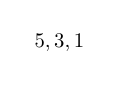
\begin{tikzpicture}[scale=.2]
\node[rectangle, scale=0.75] at (0, 0) {$\profile{5, 3, 1}$};
\end{tikzpicture}
\nodepart{two}
\footnotesize{5.625}
};
 \\ 
\\
};
\end{scope}
\begin{scope}[yshift=\leveltopIII cm, anchor = center]
\matrix (line3)[row sep=0.1cm] {
\node[draw=black, rectangle split,  rectangle split parts=2] (sn0x1c29fa0){
\nodepart{one}
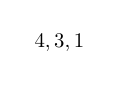
\begin{tikzpicture}[scale=.2]
\node[rectangle, scale=0.75] at (0, 0) {$\profile{4, 3, 1}$};
\end{tikzpicture}
\nodepart{two}
\footnotesize{5.125}
};
 \\ 
\\
};
\end{scope}
\begin{scope}[yshift=\leveltopIIII cm, anchor = center]
\matrix (line4)[row sep=0.1cm] {
\node[draw=black, rectangle split,  rectangle split parts=2] (sn0x1c28250){
\nodepart{one}
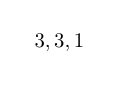
\begin{tikzpicture}[scale=.2]
\node[rectangle, scale=0.75] at (0, 0) {$\profile{3, 3, 1}$};
\end{tikzpicture}
\nodepart{two}
\footnotesize{4.625}
};
 \\ 
\\
};
\end{scope}
\begin{scope}[yshift=\leveltopIIIII cm, anchor = center]
\matrix (line5)[row sep=0.1cm] {
\node[draw=black, rectangle split,  rectangle split parts=2] (sn0x1c23d40){
\nodepart{one}
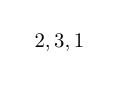
\begin{tikzpicture}[scale=.2]
\node[rectangle, scale=0.75] at (0, 0) {$\profile{2, 3, 1}$};
\end{tikzpicture}
\nodepart{two}
\footnotesize{4.125}
};
 \\ 
\\
};
\end{scope}
\begin{scope}[yshift=\leveltopIIIIII cm, anchor = center]
\matrix (line6)[row sep=0.1cm] {
\node[draw=black, rectangle split,  rectangle split parts=2] (sn0x1c23fc0){
\nodepart{one}
\begin{tikzpicture}[scale=.2]
\node[rectangle, scale=0.75] at (0, 0) {$\profile{1, 3, 1}$};
\end{tikzpicture}
\nodepart{two}
\footnotesize{3.625}
};
 \\ 
\\
};
\end{scope}
\begin{scope}[yshift=\leveltopIIIIIII cm, anchor = center]
\matrix (line7)[row sep=0.1cm] {
\node[draw=black, rectangle split,  rectangle split parts=2] (sn0x1c240d0){
\nodepart{one}
\begin{tikzpicture}[scale=.2]
\node[rectangle, scale=0.75] at (0, 0) {$\profile{1, 2, 1}$};
\end{tikzpicture}
\nodepart{two}
\footnotesize{3.25}
};
 \\ 
\node[draw=black, rectangle split,  rectangle split parts=2] (sn0x1c241e0){
\nodepart{one}
\begin{tikzpicture}[scale=.2]
\node[rectangle, scale=0.75] at (0, 0) {$\profile{3, 1}$};
\end{tikzpicture}
\nodepart{two}
\footnotesize{3}
};
 \\ 
\\
};
\end{scope}
\begin{scope}[yshift=\leveltopIIIIIIII cm, anchor = center]
\matrix (line8)[row sep=0.1cm] {
\node[draw=black, rectangle split,  rectangle split parts=2] (sn0x1c242f0){
\nodepart{one}
\begin{tikzpicture}[scale=.2]
\node[rectangle, scale=0.75] at (0, 0) {$\profile{1, 1, 1}$};
\end{tikzpicture}
\nodepart{two}
\footnotesize{3}
};
 \\ 
\node[draw=black, rectangle split,  rectangle split parts=2] (sn0x1c245b0){
\nodepart{one}
\begin{tikzpicture}[scale=.2]
\node[rectangle, scale=0.75] at (0, 0) {$\profile{2, 1}$};
\end{tikzpicture}
\nodepart{two}
\footnotesize{2.5}
};
 \\ 
\\
};
\end{scope}
\draw (sn0x1c22990.east) -- (sn0x1c28c10.west);
\draw (sn0x1c28c10.east) -- (sn0x1c29fa0.west);
\draw (sn0x1c29fa0.east) -- (sn0x1c28250.west);
\draw (sn0x1c28250.east) -- (sn0x1c23d40.west);
\draw (sn0x1c23d40.east) -- (sn0x1c23fc0.west);
\draw (sn0x1c23fc0.east) -- (sn0x1c240d0.west);
\draw (sn0x1c23fc0.east) -- (sn0x1c241e0.west);
\draw (sn0x1c240d0.east) -- (sn0x1c242f0.west);
\draw (sn0x1c240d0.east) -- (sn0x1c245b0.west);
\draw (sn0x1c241e0.east) -- (sn0x1c245b0.west);
\end{tikzpicture}
%%% Local Variables:
%%% TeX-master: "../thesis.tex"
%%% End: 
  \caption{A snapshot DAG (HLF, two processors) and its corresponding profile DAG containing much less nodes than the original snaphsot DAG. \emph{Remark:} Snapshots with same profiles have the same expected run time and can thus be merged. }
  \label{fig:p2-profile-dag-example-000111223-hlfdet}
\end{figure}

To be more mathematical: If the snapshot DAG is $(V_s, E_s)$, then the profile DAG can be expressed as $(V_p, E_p)$. These are defined as follows:
\begin{eqnarray*}
  V_p &=& \left\{ \text{PROFILE}(v) \mid v \in V_s \right\} \\
  E_p &=& \left\{ \left(\text{PROFILE}(v_1), \text{PROFILE}(v_2) \right) \mid (v_1, v_2)\in E_s\right\}
\end{eqnarray*}

The function $\text{PROFILE}$ takes a snapshot as input and returns the profile corresponding the the snapshot's intree. Note that $\text{PROFILE}$ then is a homomorphism between the snapthot and the profile DAG.\todo{Stimmt das?}

If we compute the expected run time via the profiles (as equation (\ref{eq:p2-profile-optimal-exp-run-time-def-simplified}) suggests), we only need to compute the profiles arising in the profile DAG. We can cache intermediate results, so we do not need to compute the runtime of any profile twice.

Thus, it is an important question how big these profile DAGs can get. To tackle this question, we examine for a profile $P=\profile{n_1,\dots,n_r}$ how many profiles of a certain length exist as successors of this profile.

We inspect the following example: Consider the profile $\profile{4,3,5,1}$. Its successing profiles of length 4 are
\begin{equation*}
  \profile{3, 3, 5, 1},
  \profile{2, 3, 5, 1},
  \profile{1, 3, 5, 1},
  \profile{1, 2, 5, 1},
  \profile{1, 1, 5, 1},
  \profile{1, 1, 4, 1},
  \profile{1, 1, 3, 1},
  \profile{1, 1, 2, 1} \text{ and }
  \profile{1, 1, 1, 1}.
\end{equation*}

We recognize that the first item in the succesing profiles has to be at most 4 (since the \emph{original} first entry was exactly 4). Moreover, the second entry can only be less then 3 (\emph{original} second entry: 3) if the first entry is 1. Similarily, the third entry in a successing profile can only be less then 5 (original third entry: 5) if the first and the second entry are 1.

More general: In a successing profile, the entry at a certain position can only be less than the original entry at this position if all entries \emph{up to that position} are already 1.

\begin{definition}[Successing profiles]
Let $P=\profile{n_1,\dots,n_r}$ be a profile of lenght $r$. The set of successing profiles of length $j$ of original profile $P$ is
\begin{equation*}
  S^p_{j}
  :=
  \left\{ 
    \profile{m_{r-j+1},\dots,m_{r}}
    \mid
    \exists p \in \left\{ r-j+1,\dots,r \right\}.\,
    \bigwedge_{i=1}^{p-1} m_i = 1 \ \wedge m_p < n_p
  \right\}.
  \todo{Beispiel}
\end{equation*}

The set of \emph{all} successing profiles clearly is then
\begin{equation*}
  S^P
  :=
  \bigcup_{j=1}^r S^P_j.
\end{equation*}
\end{definition}

The size of the profile DAG (starting at a certain profile $P$) is then clearly denoted by the size of $S^P$.

\begin{lemma}[Size of profile DAG]
  \label{lem:profile-dags-exact-size}
  Let $P=\profile{n_1,\dots,n_r}$ be a profile. Then, 
  \begin{equation*}
    \left| S^P \right| = 
    \sum _{j=1}^{r-1} j \cdot n_j 
    -0.5r^2 + 1.5 r.
  \end{equation*}
\end{lemma}

\begin{proof}
  If $P=\profile{n_1,\dots,n_r}$ is a profile, then the size of the set $S^P_j$ is
  \begin{equation*}
    1+ \sum_{i=j}^{r-1} (n_i-1).
  \end{equation*}
  
  In a successing profile, the entry at position $p$ can take exactly the values $1, 2, 3, \dots, n_p-1$ (where $n_p$ is th entry at positon $p$ in profile $P$). This yields the term $(n_i-1)$. Moreover, we stated that the entry at position $p$ can only be smaller if \emph{all previous entries} are 1. Thus, we can simply sum um the terms for the different positions, yielding the above sum.

  We now sum up over the different possible \emph{lengths} (ranging from 1 to $r$) of the successor profiles, and afterwards apply well-known summation rules and formulae for triangular numbers:
  \begin{eqnarray*}
    \left| S^P \right| & = & \sum_{j=1}^{r} \left( 1+ \sum_{i=j}^{r-1} (n_i-1) \right) \\
    &=& \sum_{j=1}^{r} 1 + \sum_{j=1}^{r} \left( \sum_{i=j}^{r-1} n_i \right) - \sum_{j=1}^{r}\sum_{i=j}^{r-1} 1 \\
    &=&r - \sum_{j=1}^{r}(r-j) + \sum_{j=1}^{r} \left( \sum_{i=j}^{r-1} n_i \right) \\
    &=&r - \frac{r^2-r}{2} + \sum_{j=2}^{r-1} \left( \sum_{i=j}^{r-1} n_i \right) \\
    &=&\sum _{j=1}^{r} \left( \sum _{i=j}^{r-1}n_{{i}} \right) + -0.5r^2 + 1.5 r
  \end{eqnarray*}

  It remains to be shown that $\sum _{j=1}^{r} \left( \sum _{i=j}^{r-1}n_{{i}} \right) = \sum_{j=1}^{r-1}(j-1)\cdot n_j$. This can be seen by considering the following:
  \begin{eqnarray*}
    \setlength{\arraycolsep}{2pt}
    \begin{array}{cccccccccccccccc}
      \displaystyle
      \sum_{j=2}^{r-1} \left( \sum _{i=j}^{r-1}n_{{i}} \right) &=&
         n_1 & + & n_2 & + & n_3 & + & n_4 & + & \dots & + & n_{r-2} & + & n_{r-1}  & + \\
      & &    &   & n_2 & + & n_3 & + & n_4 & + & \dots & + & n_{r-2} & + & n_{r-1}  & + \\
      & &    &   &     &   & n_3 & + & n_4 & + & \dots & + & n_{r-2} & + & n_{r-1}  & + \\
      & &    &   &     &   &     & + & n_4 & + & \dots & + & n_{r-2} & + & n_{r-1}  & + \\
      & &    &   &     &   &     &  &  &  & \ddots &  &  &  & \vdots  & + \\
      & &    &   &     &   &     &   &     &   &   &   &  n_{r-2}  & +  & n_{r-1}  & +  \\
      & &    &   &     &   &     &   &     &   &   &   &    &   & n_{r-1}  &   \\
      \\
      &=& n_1 &+& 2 n_2 & + & 3 n_3 &+& 4 n_4 &+& \dots & + & (r-2)\cdot n_{r-2} &+& (r-1)\cdot n_{r-1} & \\
    \end{array}
  \end{eqnarray*}
  This shows that $\left|S^P\right| = \sum _{j=1}^{r-1} j \cdot n_j 
    -0.5r^2 + 1.5 r$.
\end{proof}

Now that we know the size of the profile DAG, this imposes the question how many nodes a profile DAG has \emph{in the worst case} if we consider an intree with exactly $n$ tasks.

\begin{lemma}
  \label{lem:profile-dags-form-of-maximum-profile}
  For an intree with $n$ nodes and $r$ levels (i.e. an intree having a profile with $r$ entries), the maximum size of the profile DAG is reached if the profile is of the form $\profile{\profileones{r-2},n-r+1,1}$.
\end{lemma}

\begin{proof}
  We compute the number of nodes in the profile DAG for the profile $P^*= \profile{\profileones{r-2},n-r+1,1}$. According to lemma  \ref{lem:profile-dags-exact-size}, it is exactly
  \begin{equation*}
    \sum_{j=1}^{r-2} j\cdot 1 + (r-1)\cdot(n-r+1) = \frac{(r-1)\cdot(r-2)}{2} + (r-1)\cdot(n-r+1).
  \end{equation*}
  We consider now an arbitrary profile, but express it in terms of $P^*$. That is, we consider a profile $P=\profile{n_1,\dots,n_r}$, where $n_i = 1 + b_i$, for $i\in\left\{1,2,\dots,r-2\right\}$ and $n_{r-1} = (n-r+1) + b_{r-1}$. Note that this means that each $n_i$ (entry in $P$) is expressed as the corresponding entry in $P^*$ plus some constant $b_i$ chosen appropriately. Of course $n_r = 1$.

  Two observations are important now:

  \begin{itemize}
  \item Since all $n_i \in \naturals$, we can condlude that $b_i \geq 0$ for $i\in\{1,2,\dots,r-2\}$.
  \item Since the number of all tasks has to be the same, we know that $P^*$ and $P$ must have the same number of tasks (namely $n$). This means that
    \begin{equation*}
      n = \sum_{i=1}^r n_i = \sum_{i=1}^{r-2} \left[ 1+b_i \right] + \left[(n-r+1)+b_{r-1} \right] + 1.
    \end{equation*}
    We simplify the above to
    \begin{equation*}
      \sum_{i=1}^{r-2} \left[ 1+b_i \right] + \left[(n-r+1)+b_{r-1} \right] + 1 =
      \sum_{i=1}^{r-2} b_i + r-2 + n-r+1+b_{r-1}+1 = 
      n + \sum_{i=1}^{r-1} b_i
    \end{equation*}
    From this we can conclude that $b_{r-1} = -(\sum_{i=1}^{r-2})$.
  \end{itemize}

  We can now compute the number of nodes for profile $P$ (remember: an arbitrary profile expressed through $P^*$ and the $b_i$'s):

  \begin{eqnarray*}
    \sum_{j=1}^{r-1} j \cdot n_j &=& \sum_{j=1}^{r-2} j\cdot (1+b_j) + (r-1)(n-r+1+b_{r-1}) \\
    &=& \sum_{j=1}^{r-2} j + \sum_{j=1}^{r-2} j\cdot b_j + (r-1)\left(n-r+1-(\sum_{j=1}^{r-2} b_j)\right) \\
    &=& \frac{(r-2)\cdot(r-1)}{2} + (r-1)(n-r+1) + \sum_{j=1}^{r-2} j\cdot b_j - \sum_{j=1}^{r-2} (r-1) \cdot b_j \\
    &=& \underbrace{\frac{(r-2)\cdot(r-1)}{2} + (r-1)(n-r+1)}_{\text{Number of nodes in DAG for $P^*$}} + \sum_{j=1}^{r-2} b_j \cdot (j-r+1) \\
  \end{eqnarray*}
  
  We recognize that the result contains the number of nodes in a profile DAG for profile $P^*=\profile{\profileones{r-2},n-r+1,1}$ --- and some additional term (namely $\sum_{j=1}^{r-2} b_j \cdot (j-r+1)$).

  However, in this term we can see that $(j-r+1) < 0$ (since $j$ ranges from 1 to r-2). This means, that the whole sum $\sum_{j=1}^{r-2} b_j \cdot (j-r+1) \leq 0$ (since all $b_j$ are positive for $j\in\left\{ 1,2,\dots,r-2\right\}$). That means, this sum gets 0 \emph{if and only if} all $b_j$ are 0 for $j\in\left\{ 1,2,\dots,r-2\right\}$.

  This, however, proves that the profile $P^*$ is the profile with exactly $r$ entries and $n$ tasks that maximizes the number of nodes in the profile DAG.
\end{proof}

It remains to explain how to choose $r$ in a way such that given the number of tasks $n$, we can construct a profile with $r$ entries such that the resulting profile DAG has the maximum number of nodes over \emph{all} intrees with $n$ tasks.

\begin{lemma}[Structure of worst-case profile]
  \label{lemma:worst-case-profile-structure}
  Given a natural number $n$, the profile maximizing the number of nodes in the profile DAG is of the form $P^*=\profile{\profileones{r-2},n-r+1,1}$, where $r$ is either $\lfloor n/2\rfloor$ or $\lceil n/2 \rceil$ (one of both --- can be chosen at will).
\end{lemma}

\begin{proof}
  The fact that the profile maximum the number of nodes in the profile DAG is of the form $\profile{\profileones{r-2},n-r+1,1}$ follows directly from lemma \ref{lem:profile-dags-form-of-maximum-profile}. Thus, we can restrict ourselves onto those if we look for profiles maximizing the number of nodes in a profile DAG for a certain number of tasks.
  
  We consider the number of nodes in a profile DAG for a profile of the form $\profile{\profileones{r-2},n-r+1,1}$, given by lemma \ref{lem:profile-dags-exact-size}:
  \begin{equation*}
    \sum_{j=1}^{r-2} j \cdot 1 + (r-1)\cdot(n-r+1) -0.5r^2 +1.5r = \frac{(r-2)\cdot(r-1)}{2} + (r-1)\cdot(n-r+1) -0.5r^2 +1.5r
  \end{equation*}

  Our goal is now to maximize this term by choosing $r$ accordingly depending on $n$. We simplify the above to
  \begin{equation*}
    r+r \left( n-r+1 \right) -1 = -r^2+r\cdot(n+2)-1
  \end{equation*}
  and recognize that this is a downward opened parabola having the derivative
  \begin{equation*}
    3+n-2r,
  \end{equation*}
  meaning that its maximum is at $r=\frac{n+2}{2}$. Since this is only a natural number if $n$ is even and since we have -- as said before -- a parabola, we can simply apply rounding to get the maximum for natural-values. This means, we can derive natural solution: $r^*=\lfloor \frac{n+2}{2} \rfloor$ or $r^*=\lceil \frac{n+2}{2} \rceil$ (can be chosen at will since we have a parabola). Without loss of generality, we focus on $r^*=\lfloor \frac{n+2}{2} \rfloor = \lfloor\frac{n}{2} \rfloor + 1$.

  This means that the profile DAG has a maximum of nodes if we consider the profile
  \begin{equation*}
    \profile{\profileones{r^*-2},n-r^*+1,1} = 
    \profile{
      \profileones{\left( \left\lfloor\frac{n}{2} \right\rfloor + 1 \right)-2},
      n-\left( \left\lfloor\frac{n}{2} \right\rfloor + 1 \right)+1,
      1
    } = 
    \profile{
      \profileones{ \left\lfloor\frac{n}{2} \right\rfloor - 1},
      \left\lceil \frac{n}{2} \right\rceil,
      1
    } 
  \end{equation*}
  Similarily, we could have chosen $r^*=\lceil\frac{n}{2}\rceil+1$. This shows the claim.
\end{proof}

We can now combine the lemmata to the following theorem:

\begin{theorem}[Size of snapshot DAG]
  For an intree with exactly $n$ tasks, the profile DAG has at most $\lfloor \frac{n}{2} \rfloor \cdot \lceil \frac{n}{2} \rceil +1$ nodes.
\end{theorem}

\begin{proof}
  Lemma \ref{lemma:worst-case-profile-structure} gives us that the wors-case profile is $P^*=\profile{ \profileones{ \left\lfloor\frac{n}{2} \right\rfloor - 1}, \left\lceil \frac{n}{2} \right\rceil, 1 }$, which we use to compute the number of nodes in the corresponding worst-case profile DAG according to lemma \ref{lem:profile-dags-exact-size}:
  \renewcommand{\r}{\left(\left\lfloor\frac{n}{2}\right\rfloor + 1\right)}
  \begin{equation*}
    \frac{(\r-2)\cdot(\r-1)}{2} + 
    \left(\r-1\right)\cdot\left( \left\lceil \frac{n}{2} \right\rceil \right)
    - \frac{1}{2} \cdot \r^2 + \frac{3}{2} \cdot \r     
  \end{equation*}
  We simplify the above to
  \newcommand{\ceiln}{\left\lceil \frac{n}{2} \right\rceil}
  \newcommand{\floorn}{\left\lfloor \frac{n}{2} \right\rfloor}
  \begin{eqnarray*}
    \frac{\left( \floorn -1 \right)\left( \floorn \right)}{2}
    + \floorn \cdot \ceiln
    - \frac{\floorn^2 + 2\cdot \floorn + 1}{2}
    + \frac{3\cdot \floorn + 3}{2}
    & = &
    \ceiln \cdot \floorn + 1,
  \end{eqnarray*}
  proving the claim.
\end{proof}

%%% Local Variables:
%%% TeX-master: "../thesis.tex"
%%% End: 